\documentclass[10pt]{article}
\usepackage[left=2.5cm,right=2.5cm,top=2cm,bottom=2cm]{geometry}
% -------------------------------------------------------------------
\usepackage[english]{babel}
\usepackage[utf8]{inputenc}									
\usepackage[T1]{fontenc}										% 
% -------------------------------------------------------------------
\usepackage{amsmath,amsfonts,amssymb,amsthm,cancel,siunitx,
calculator,calc,mathtools,empheq,latexsym}
\usepackage[version=4]{mhchem}
\usepackage[official]{eurosym}
% -------------------------------------------------------------------
\usepackage{subcaption,epsfig,tikz,float}
\usepackage{xcolor}
\usepackage{booktabs,multicol,multirow,tabularx,array}
\usepackage{multicol}
\usepackage{lipsum}
\usepackage{csquotes}
\usepackage[super]{nth}
\usepackage[numbers]{natbib}
\usepackage{xurl}
\usepackage[breaklinks]{hyperref}
\urlstyle{same}
\hypersetup{
    colorlinks,
    breaklinks=true,
    linkcolor={black!50!black},
    citecolor={blue!50!blue},
    urlcolor={blue!80!blue}
}
	

% Commands
\newcommand*{\doi}[1]{\href{http://dx.doi.org/#1}{doi: #1}}

% Aliases
\let\autocite\cite

% -------------------------------------------------------------------
\setlength{\parindent}{0pt}
\setlength{\parskip}{5pt}
% \textheight 19.5cm
\columnsep .5cm
% -------------------------------------------------------------------
\title{\renewcommand{\baselinestretch}{1.17}\normalsize\bf%
\uppercase{The Role of Projects of Common Interest\\in Reaching European Energy Policy Targets}\\--- working title ---
}
% -------------------------------------------------------------------
% Authos
\author{%s
Bobby Xiong$^{1,*}$, Iegor Riepin$^{1}$, Tom Brown$^{1}$\\ 
}
\date{}
% -------------------------------------------------------------------

% GRAPHICS	
\graphicspath{
    {graphics/}
  }
\DeclareGraphicsExtensions{.pdf,.jpeg,.png,.jpg}


\begin{document}

\maketitle

\vspace{-1cm}

\begin{center}
{\footnotesize 
$^1$Technische Universität Berlin, Department of Digital Transformation in Energy Systems, Germany \\
$^*$Presenting author: \href{mailto:xiong@tu-berlin.de}{xiong@tu-berlin.de}
}\\
\smallskip
\footnotesize
\textbf{Tags}: resilience, infrastructure, energy system modelling, energy policy \\
\medskip
\textbf{\nth{43} International Energy Workshop --- relevant conference topics:}\\(1) Reaching net-zero emissions and climate neutrality \textbullet{} (2) Role of renewable energy in the energy transition \textbullet{} (3) Role of hydrogen, ammonia, e-fuels and e-methane in the energy transition \textbullet{} (4) Managing power system transitions --- integration of variable renewable energy and power-to-X \textbullet{} (5) Sectoral pathways for the energy transition --- transport, industry, and buildings \textbullet{} (6) Energy transition infrastructure --- assessment of infrastructure to enable the energy transition, including electrical transmission, storage, EV charging, and hydrogen distribution, CCS and CDR \textbullet{} (12) Climate resilience of energy systems \textbullet{} (13) Utilisation of scenarios by governments
\end{center}

% -------------------------------------------------------------------

\section*{Summary}
% 100-200 words

Summary

\section*{Introduction and motivation}

On the pathway to a climate-neutral by 2050, the European Union (EU) has set ambitious targets for 2030, three of the most prominent including \SI{55}{\percent} greenhouse gas emission reduction \autocite{europeancommissionFit55Delivering2021}, \SI{10}{Mt} p.a. green \ce{H2} production \autocite{europeancommissionREPowerEUPlanCommunication2022}, and \SI{50}{Mt} p.a. \ce{CO2} sequestration \autocite{europeanparliamentRegulationEU20242024}. 

To support reaching these targets, the EU has identified a list of Projects of Common Interest (PCI) which are key cross-border infrastructure projects that link the energy systems of EU countries, ranging from storages, over transmission lines to pipelines and carbon sinks \autocite{europeancommissionCommissionDelegatedRegulation2023}. Projects of Mutual Interest (PMI) further include cooperations with countries outside the EU, such as the United Kingdom. In order for projects to be eligible for PCI-PMI status, their potential benefits need to outweigh their costs \autocite{europeancommissionCommissionDelegatedRegulation2023}. Given the political and lighthouse character, these projects are highly likely to be implemented. However, any large infrastructure project, including PCI-PMI projects, are commonly facing delays due to permitting, financing, procurement bottlenecks, etc. \autocite{acerConsolidatedReportProgress2023}.

From the ambitious policy targets and the nature of PCI-PMI projects, we derive the following key research questions:

\begin{enumerate}
    \item At what cost do we stick to reaching the EU policy targets?
    \item How does a delay of PCI-PMI projects affect the system, its costs, and the ability to reach the EU policy targets?
    \item What is the impact of missing the EU 2030 policy targets for \ce{CO2} sequestration and \ce{H2} production?
 \end{enumerate}

\section*{Methodology}

We use the open-source, sector-coupled energy system model PyPSA-Eur \autocite{horschPyPSAEurOpenOptimisation2018} to optimise investment into generation, storage, and transmission infrastructure (including electricity, natural gas, hydrogen, \ce{CO2}, and Power-to-X conversion) as well as operation/dispatch. The model is spatially and temporally highly resolved and covers the entire European continent, including stocks of existing power plants, renewable potentials, and availability time series. It covers today's high-voltage transmission grid (AC \SI{220}{kV} to \SI{750}{kV} and DC \SI{150}{kV} upwards) \autocite{xiongModellingHighVoltageGrid2024}.

\paragraph{Feature implementation} By accessing the REST API of the PCI-PMI Transparency Platform \autocite{europeancommissionPCIPMITransparencyPlatform2024} and associated public project sheets provided by the European Commission, we implement the PCI-PMI projects into the PyPSA-Eur model to assess their impact in the power, heat, transport, industry, feedstock, and agriculture sector. Our implementation can adapt to the needs and configuration of the model, including selected technologies, geographical and temporal resolution, as well as the level of sector-coupling. An overview of the implemented PCI-PMI projects is shown in Figure \ref{fig:pci_pmi_projects_map}.

\begin{figure}[!htbp]
    \centering
    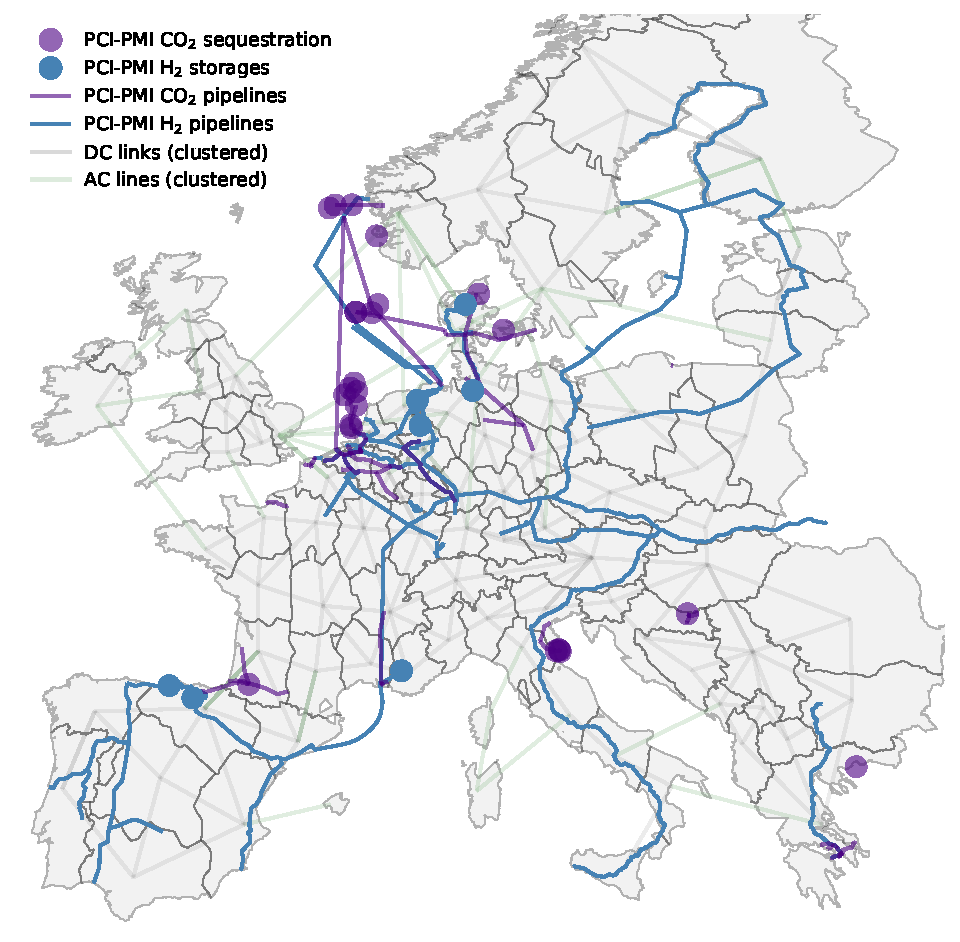
\includegraphics[width=0.55\textwidth]{pci_pmi_projects_map}
    \caption{PCI-PMI projects implemented in the PyPSA-Eur model. Own illustration based on data from the European Commission \autocite{europeancommissionPCIPMITransparencyPlatform2024}.}
    \label{fig:pci_pmi_projects_map}
\end{figure}

\paragraph{Scenario setup} As of the date of submission, we model three key scenarios for the target year 2030 which will set the base year for pathways towards 2050: a `Base' scenario in which all all projects are commissioned on time and policy targets are achieved and two PCI-PMI delay scenarios `A' and `B'. Table \ref{tab:scenarios} gives an overview of the scenarios' key assumptions.

\begin{table}[!htbp]
    \centering
    \caption{Scenarios setup. Own illustration.}
    \begin{tabular}{lccc}
        \toprule
        Assumption \textbackslash{} Scenario & Base & A. All targets & B. Emission target only \\
        \midrule
        PCI-PMI projects & on time & delayed & delayed \\
        \midrule
        \ce{CO2} emission target & \SI{-55}{\percent}/\SI{2}{Gt} p.a. & \SI{-55}{\percent}/\SI{2}{Gt} p.a. & \SI{-55}{\percent}/\SI{2}{Gt} p.a. \\
        \ce{CO2} sequestration target & \SI{50}{Mt} p.a. & \SI{50}{Mt} p.a. & --- \\
        \ce{H2} target & \SI{10}{Mt} p.a. & \SI{10}{Mt} p.a. & --- \\
        \midrule
        \ce{CO2} sequestration sites & PCI-PMI & endogeneous & endogeneous \\
        \ce{CO2} pipelines & PCI-PMI + endogen. expansion & --- & --- \\
        \ce{H2} storage & PCI-PMI & endogeneous & endogeneous \\
        \ce{H2} pipelines & PCI-PMI +  endogen. expansion & --- & --- \\
        AC and DC transmission & PCI-PMI & --- & --- \\
        \bottomrule
    \end{tabular}
    \label{tab:scenarios}
\end{table}

\paragraph{Solving} We solve all scenarios by minimising total system costs, resolving 34 countries to 90 buses at 3-hourly temporal resolution.

\section*{Results (preliminary)}
First results for the modelling year 2030 show that reaching the EU's 2030 \ce{H2} production and \ce{CO2} sequestration targets translates into around 20 bn. \euro{} p.a. in total system costs for all included sectors, with or without PCI-PMI infrastructure projects (see Figure \ref{fig:system_costs}).

\begin{figure}[!htbp]
    \centering
    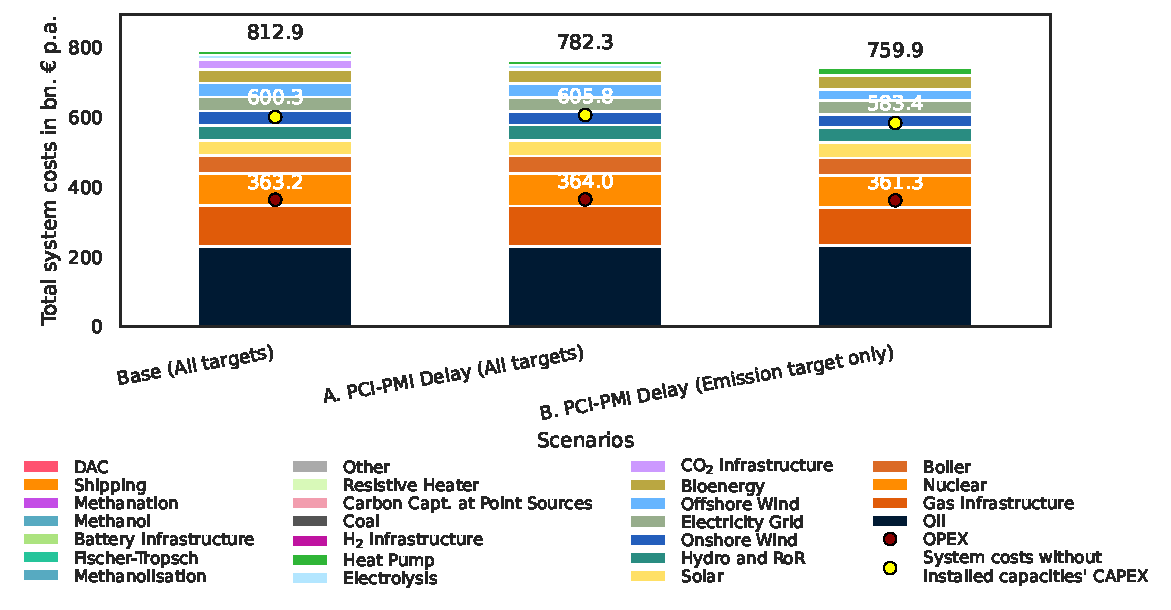
\includegraphics[width=1\textwidth]{system_costs}
    \caption{Results --- Total system costs by technology and infrastructure. Own illustration.}
    \label{fig:system_costs}
\end{figure}

By omitting an \ce{H2} target, almost no electrolysers are installed. Around \SI{8}{Mt} are still produced to cover industrial \ce{H2} and methanol (primarily shipping) demand. However, this demand is met by decentral steam methane reforming instead of electrolysers. Setting an \ce{H2} target may however be essential to kick-start the \ce{H2} economy. \ce{H2} is then primarily produced through electrolysis and used as a precursor for methanolisation to meet industrial and shipping demand.

Without specifying a \ce{CO2} sequestration target, the system still captures and sequesters around \SI{21}{Mt} of \ce{CO2} p.a. primarily from process emissions in the industry sector. 

\begin{figure}[h!]
    \centering
    \begin{subfigure}[t]{0.495\textwidth} % [t] aligns at the top
        \vspace{0pt}
        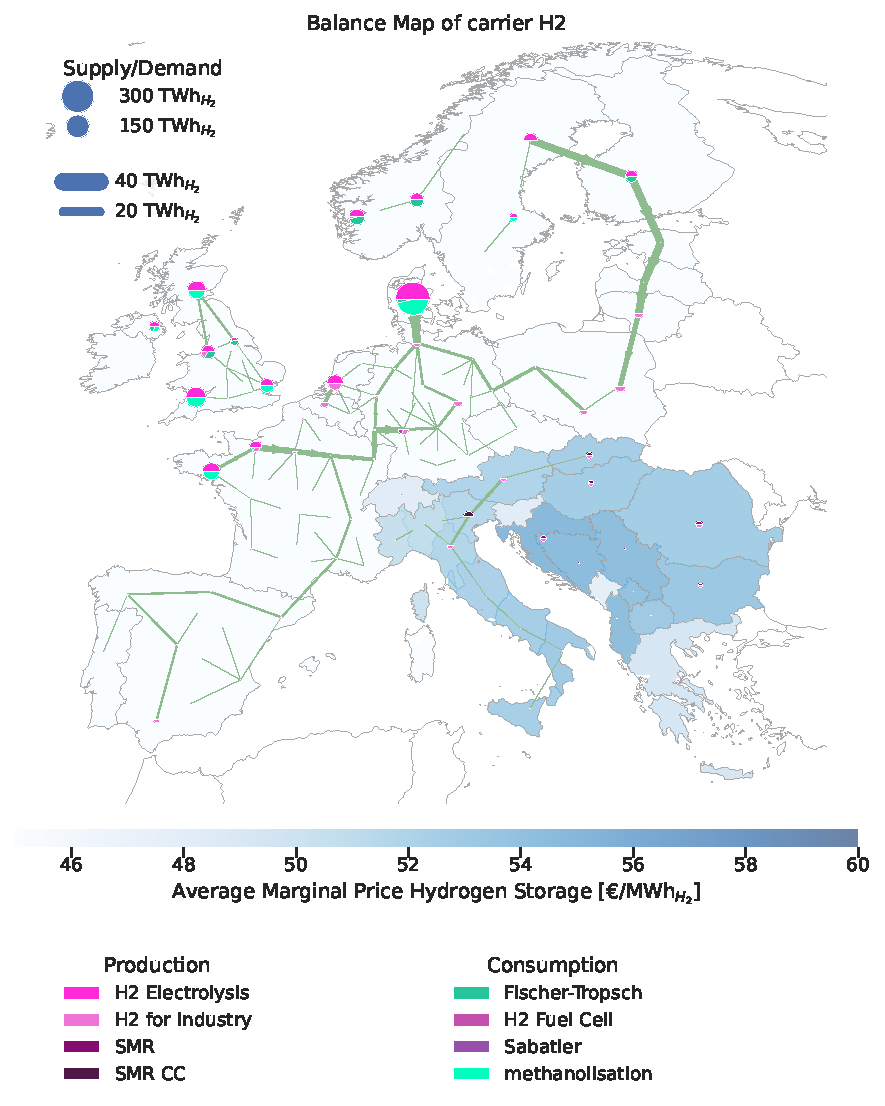
\includegraphics[width=\textwidth]{balance_map_h2} % Replace with your image
        \caption{\ce{H2} regional balances and flows.}
        \label{fig:balance_map_h2}
    \end{subfigure}
    \hfill
    \begin{subfigure}[t]{0.495\textwidth} % [t] aligns at the top
        \vspace{0pt}
        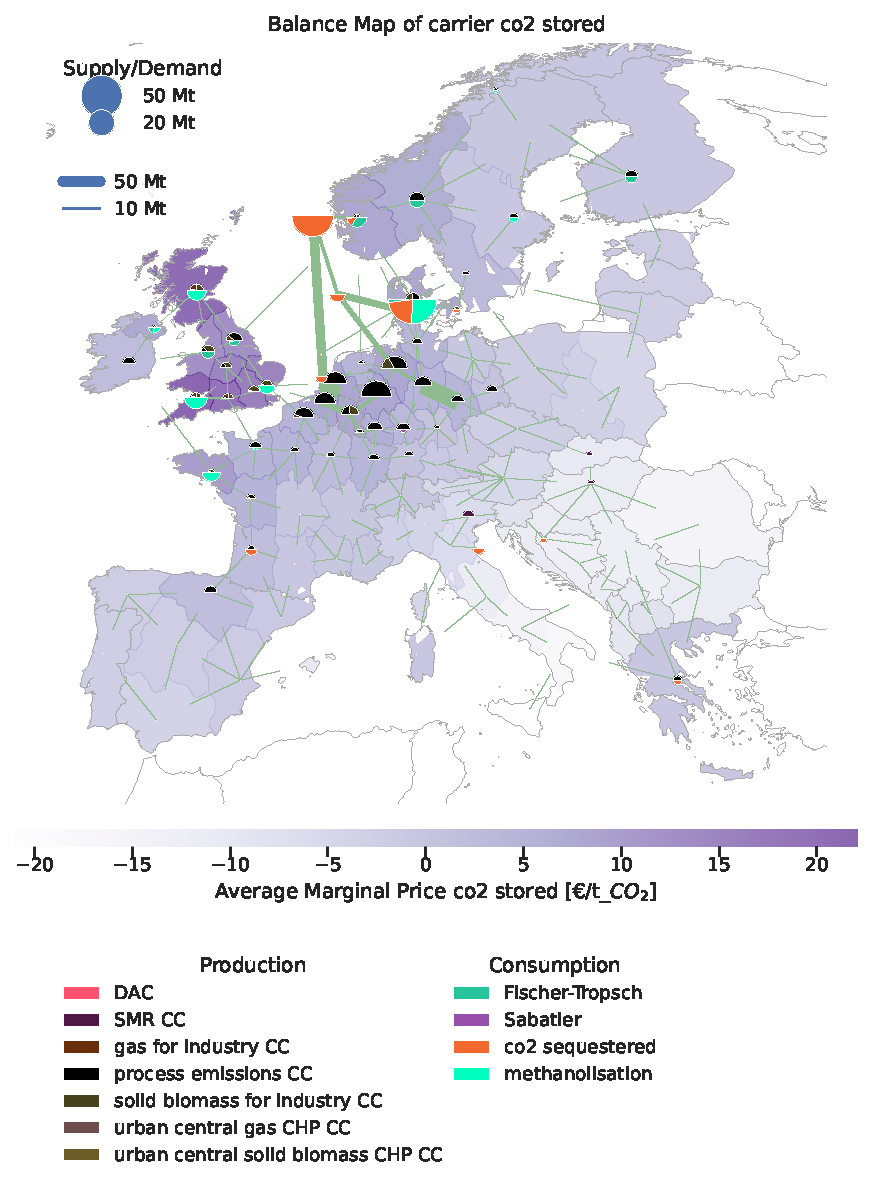
\includegraphics[width=\textwidth]{balance_map_co2} % Replace with your image
        \caption{\ce{CO2} regional balances and flows.}
        \label{fig:balance_map_co2}
    \end{subfigure}
    \caption{Results --- Regional distribution of \ce{H2} and \ce{CO2} production, utilisation, storage, and transport. Own illustration.}
    \label{fig:balance_maps}
\end{figure}

\newpage
\section*{Conclusion (preliminary)}
We conclude that while all three EU policy targets for 2030 can be achieved without PCI-PMI infrastructure, they bring additional benefits: i) \ce{H2} pipelines projects help distribute more affordable green H$_2$ from northern and south-western Europe to high-demand regions in central Europe; ii) \ce{CO2} transport and storage projects help decarbonising the industry by connecting major industrial sites and their process emissions to offshore sequestration sites in the North Sea (Denmark, Norway, and the Netherlands).

\paragraph{Research outlook} Next steps include the implementation of remaining PCI-PMI projects, such as hybrid offshore interconnectors (energy islands), electricity storages, and \ce{CO2} shipping routes. To evaluate the long-term value of PCI-PMI projects in a sector-coupled European energy system, we will model pathway dependencies towards 2050. We will also assess the sensitivity of the infrastructure to technology-specific build-out rates.

% % -----------------------------

\bibliographystyle{plainnat}
\bibliography{references.bib}

\end{document}